\documentclass{article}
\usepackage[english]{babel}
\usepackage[utf8]{inputenc}
\usepackage{graphicx}
\usepackage{titletoc}
\usepackage[section]{placeins}
\usepackage{siunitx}
\usepackage{amsmath}
\usepackage{caption}
\usepackage{fancyhdr}
\usepackage{tabto}
\usepackage{listings}

\pagestyle{fancy}
\fancyhf{}
\rhead{Schäfer, Schnöll}
\lhead{EPH Labor}
\rfoot{Seite \thepage}

\begin{document}

\tableofcontents

\newpage
\section{Inventarliste}
  \begin{itemize}
    \item Raspberry Pi 3
    \item Potentiometer Rx 10k \si{\ohm}
    \item MCP3008 (Analog-Digital Converter)
    \item Widerstand R1 1000 \si{\ohm}
    \item Kondensator C1 47$\mu$F
  \end{itemize}

\newpage
\section{Strom- / Spannungsmessung und Verlauf aufnehmen mittels Raspberry Pi}
In dieser Laborübung ging es um die Aufnahme von analogen Signalen und deren digitale Verarbeitung mithilfe des Raspberry Pi.
Als analoge Signale dienen einerseits ein Spannungsabfall über einem Potentiometer sowie die Lade- und Entladekurve eines Kondensators.

\subsection{Vorbereitung}
Als Vorbereitung für das Labor wurde der Raspberry Pi konfiguriert und ein C-Programm für die Behandlung der digitalen Inputs erstellt.
Weiteres wurde das Datenblatt für den Analog-Digital Converter MCP3008 (fortfolgend ADC) heruntergeladen.
Die Pinbelegung ist in Figure~\ref{fig:ADCPinbelegung} ersichtlich.

\begin{figure}[h!]
    \centering
    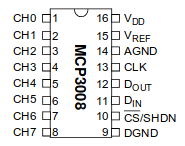
\includegraphics[width=0.4\textwidth]{MCP3008-Pinbelegung.png}
    \caption{Pinbelegung MCP3008}
    \label{fig:ADCPinbelegung}
\end{figure}

\newpage
\subsection{ADC an den Raspberry Pi anschließen}
Der MCP3008 ermöglicht die Verarbeitung von acht analogen Signalen. Diese können an die linke Seite des ADC angeschlossen werden.
Am Raspberry Pi muss die Hardware SPI Schnittstelle aktiviert werden.
Danach ist es möglich mittels der \textit{wiringPi.h} Library die Schnittstelle anzusteuern.
Die Verkabelung ist in Figure~\ref{fig:ADC-Verkabelung} visualisiert.

\begin{figure}[h!]
    \centering
    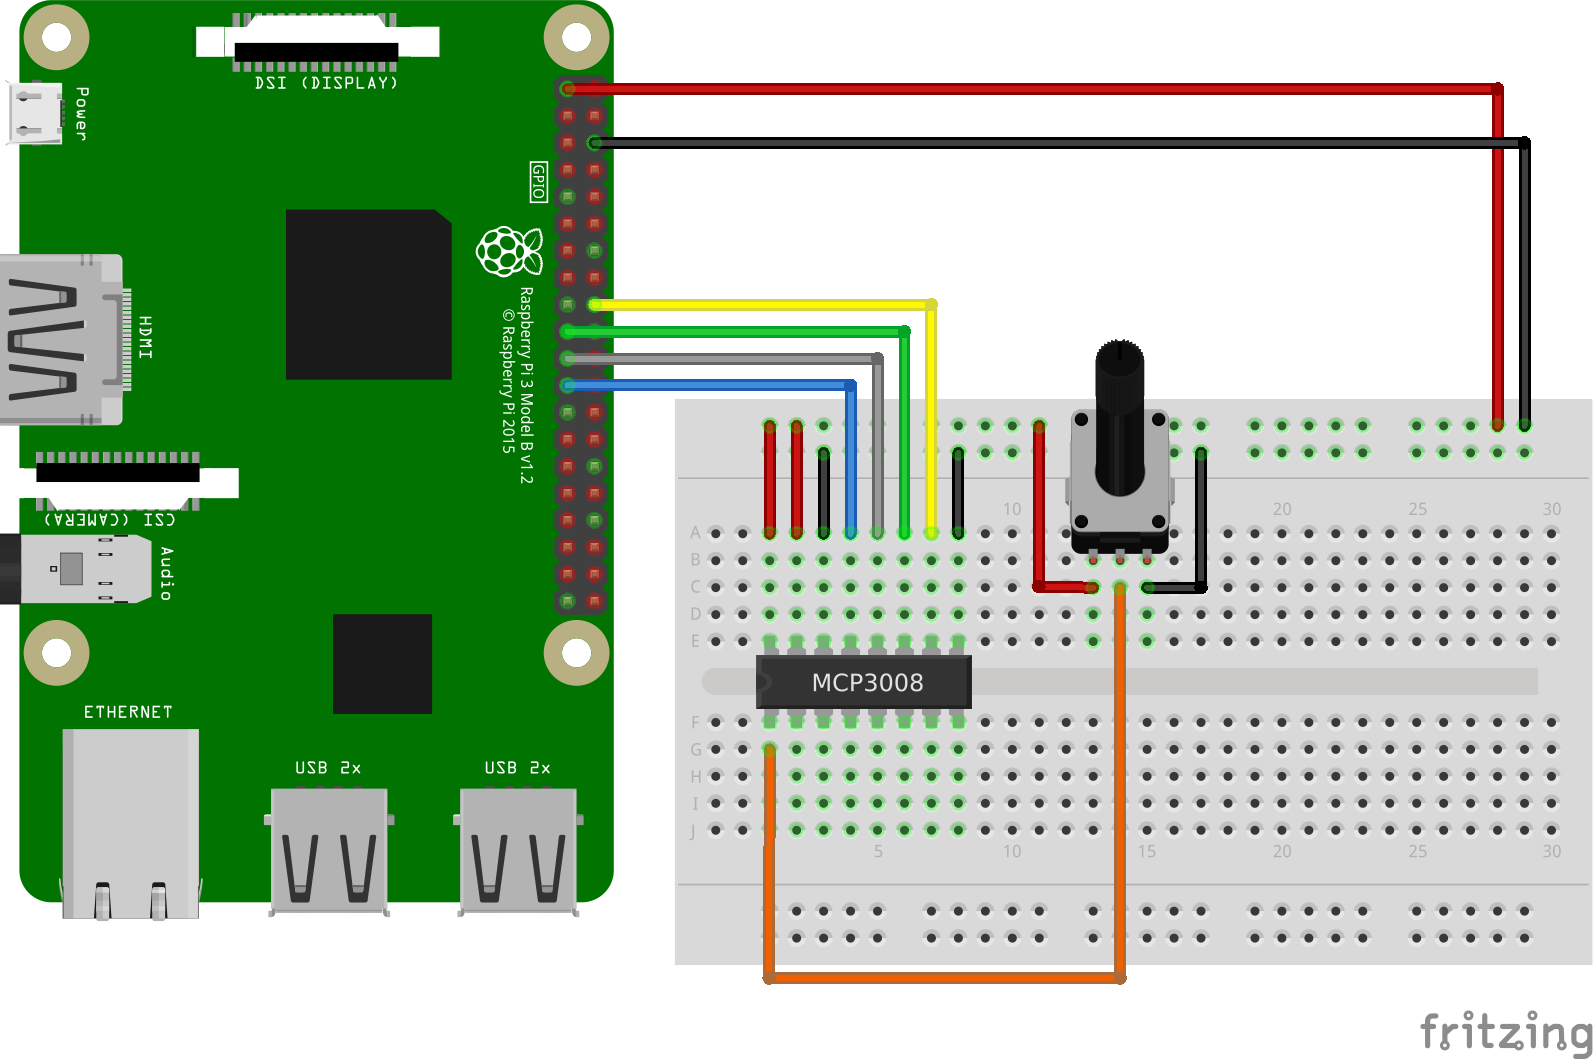
\includegraphics[width=0.8\textwidth]{RPi-Fritzing-Potentiometer_bb.png}
    \caption{Verkabelung mit dem Raspberry Pi}
    \label{fig:ADC-Verkabelung}
\end{figure}

\subsection{Berechnung des Vorwiderstandes}
Als Vorgabe wurde verlangt, dass innerhalb von $\tau$ 1/5 der Messwerte liegen. 
Insgesamt sollten 1024 Messwerte mit einem Interval von 250 $\mu$s aufgenommen werden.
Die Berechnungen sind in nachfolgender Formel aufgeführt:

\begin{align*}
    \tau &=\frac{1024}{5} * 250\mu s\\
    \tau &=0.051s\\
\end{align*}
Der Kondenstator wurde mit ($c=47\mu F$) vorgegeben. Dadurch ergibt sich für den ohmschen Widerstand ungefähr 1000$\Omega$.
\begin{align*}
    R &= \frac{\tau}{c}\\
    R &= 1089,36\Omega\\
\end{align*}

\newpage

Die Pin Verkabelung des Raspberry Pis mit dem MCP3008 wird in nachstehender Tabelle \ref{tab:Verkabelung} dargestellt. 
\begin{table}[h!]
    \begin{tabular}{|l|l|l|l|l|}
    \hline
    \multicolumn{2}{|l|}{\textbf{MCP3008}} & \multicolumn{2}{l|}{\textbf{Raspberry Pi}} & \textbf{Bemerkung}         \\ \hline
    Pin         & Signal          & Pin         & Signal              &                            \\ \hline
    16          & VDD             & 1           & 3v3                 &                            \\ \hline
    15          & VREF            & 1           & 3v3                 &                            \\ \hline
    14          & AGND            & 6           & GND                 &                            \\ \hline
    13          & CLK             & 23          & SCLK                & Clock Synchronization      \\ \hline
    12          & DOUT            & 21          & GPIO9 MISO          & Master-In Slave-Out        \\ \hline
    11          & DIN             & 19          & GPIO10 MOSI         & Master-Out Slave-In        \\ \hline
    10          & CS/SHDN         & 24          & GPIO24 CE0          & Chip Enable (Slave Select) \\ \hline
    9           & DGND            & 6           & GND                 &                            \\ \hline
    \end{tabular}
    \caption{Pin Mapping}
    \label{tab:Verkabelung}
\end{table}

\newpage
\subsubsection{Kontrollfragen}

\textbf{Was macht ein ADC? Für was wird er verwendet?}
\begin{itemize}
    \item sehr kluge Antwort
\end{itemize}
\textbf{Finden Sie die wichtigsten Kenngrößen des verwendeten ADCS MCP3004/3008 heraus.}
\begin{itemize}
    \item sehr kluge Antwort
\end{itemize}
\textbf{Was sind die Channels am ADC?}
\begin{itemize}
    \item sehr kluge Antwort
\end{itemize}
\textbf{Was ist eine SPI Schnittstelle?}
\begin{itemize}
    \item sehr kluge Antwort
\end{itemize}
\textbf{Wie funktioniert die SPI Schnittstelle?}
\begin{itemize}
    \item sehr kluge Antwort
\end{itemize}
\textbf{Was ist ein Channel (Kommunikation, zb. SPI-Channel)}
\begin{itemize}
    \item sehr kluge Antwort
\end{itemize}

\newpage

\subsection{Spannungsmessung mit ADC und Potentiometer}
Die Verkablung mit dem Potentiometer wurde abgeschlossen. Als nächstes wurde ein Programm entwickelt, 
welches die SPI Schnittstelle anspricht und die ausgelesenen Werte, neben der Ausgabe in der Konsole, in einer Datei abspeichert.t.
Um den Messvorgang zu starten wird der GPIO-Pin 26 auf HIGH geschalten. Dieser liefert 3.3 Volt an die Schaltung und versorgt den Kondensator.\\
Um die Messungen zeitlich nicht zu sehr beeinflussen, werden die Werte zuerst in eine Liste gespeichert und danach in eine Datei ausgelagert.\\
Die gemessenen Werte wurden in folgenden Format in der Datei \textit{f\_charge\_voltage.log} abgespeichert:

\noindent
Counter: fortlaufender Zeilenindex\\
Value: gemessene Spannung in Volt

\begin{lstlisting}
Counter Value
0	0.045161
1	0.061290
2	0.077419
...
1021	3.212903
1022	3.216129
1023	3.219355
\end{lstlisting}

\subsection{Berechnung des Stroms}
Zusätzlich musste der geflossene Strom ermittelt werden. Da es nicht möglich ist, mit dem ADC direkt den Strom zu messen, wird dieser berechnet.
Folgende Formel wurde für die Berechnung des Ladestroms am Kondensator verwendet:

\begin{equation}
    i=\frac{U}{R} * e^{-\frac{t}{\tau}}
\end{equation}

Gilt es den Strom der Entladekurve zu berechnen, wird folgende Formel angewandt:
\begin{equation}
    i=-\frac{U}{R} * e^{-\frac{t}{\tau}}\\
\end{equation}

wobei:
\begin{table}[h!]
    \begin{tabular}{lll}
    $i$ & ...      & Strom (Ampere            \\
    $U$ & ...      & Spannung (Volt)          \\
    $R$ & ...     & Widerstand (Ohm)         \\
    $s$ & ...     & Zeit (Sekunden)          \\
    $\tau$ & ... & Zeitkonstante (Sekunden)
    \end{tabular}
\end{table}
\newpage

Die Stromwerte werden ebenfalls zuerst in einer Liste gespeichert und danach in eine Datei geschrieben.
Der Vorgang wird für die Entladekurve des Kondensators wiederholt.\\
Um den Entladevorgang des Kondensators zu starten wird der GPIO Pin 26 auf LOW geschalten. 
Dadurch wird die Versorgungsspannung unterbrochen und der Kondensator entlädt sich am Widerstand.\\
Die Strom- und Spannungswerte werden aufgezeichnet und in die Dateien \textit{f\_discharge\_voltage.log} und \textit{f\_discharge\_current.log} geschrieben.

\subsubsection{Visualiserung mittels \textit{gnuplot}}
Um die Messwerte der Ent- und Ladekurve visuell darzustellen, bediente man sich dem Programm \textit{gnuplot}. 
Dies ermöglicht es, Dateien einzulesen und Werte in einem XY Diagramm darzustellen. \\

\paragraph{Ladekurve}\mbox{}\\
In Figure~\ref{fig:Ladekurve} kann man die Ladekurve des Kondensators deutlich erkennen. 
Der Strom ist am Anfang hoch, verringert sich jedoch nach einer Zeit, da die Kapazität des Kondensators mehr und mehr ansteigt.
\begin{figure}[h!]
    \centering
    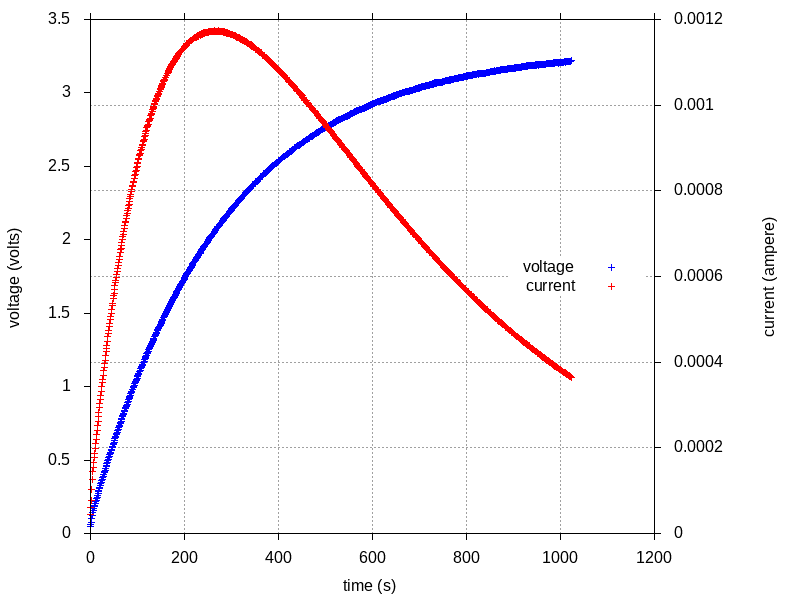
\includegraphics[width=0.8\textwidth]{rc_charging_curve_voltage_current.png}
    \caption{Ladekurve Kondensator}
    \label{fig:Ladekurve}
\end{figure}

\newpage
\paragraph{Entladekurve}\mbox{}\\
Die Entladung wird in Figure~\ref{fig:Entladekurve} festgehalten. 
Die Y-Achse des Stroms ist invertiert, man erkennt deutlich wie der Strom im Verhältnis zur abklingenden Spannung gegen 0 geht.

\begin{figure}[h!]
    \centering
    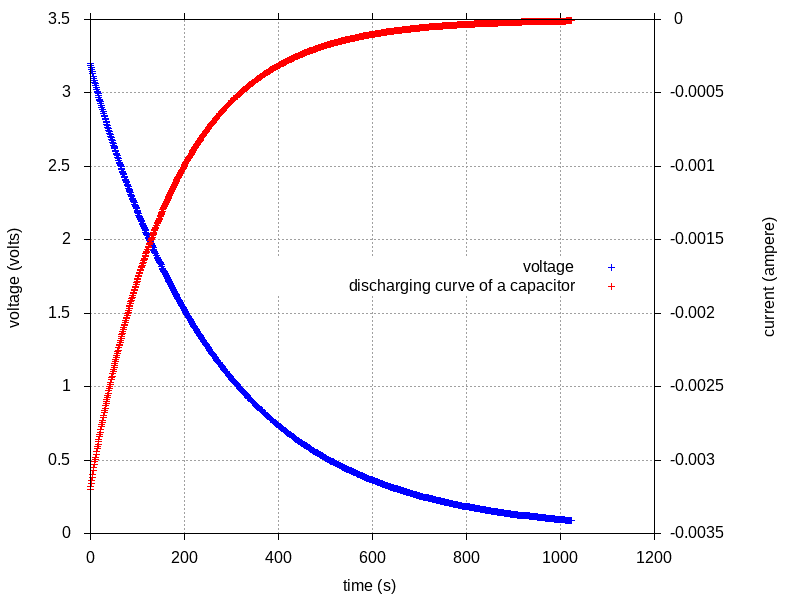
\includegraphics[width=0.8\textwidth]{rc_discharging_curve_voltage_current.png}
    \caption{Entladekurve Kondensator}
    \label{fig:Entladekurve}
\end{figure}

\subsubsection{Kontrollfragen}

\textbf{In welchen Bereich bewegen sich die Werte? Warum ist das so?}
\begin{itemize}
    \item sehr kluge Antwort
\end{itemize}
\textbf{Stellen Sie eine Formel für die Umrechnung des ADC-Wertes in einen Spannungswert auf.}
\begin{itemize}
    \item sehr kluge Antwort
\end{itemize}


\newpage
\listoffigures

\listoftables

\end{document}